\documentclass{article}
\usepackage{amsmath}
\usepackage{amssymb}
\usepackage{graphicx}
\usepackage{tikz}
\usepackage{pgfplots}
\pgfplotsset{compat=1.18}
\usepackage{booktabs}
\usepackage{xcolor}

% Custom environments
\newenvironment{lesson-meta}{}{}
\newenvironment{item-analysis}{}{}
\newenvironment{model-discuss}{}{}
\newenvironment{concept-box}{}{}
\newenvironment{concept-summary}{}{}
\newenvironment{example}[1]{\textbf{EXAMPLE #1}\par}{\par}
\newenvironment{tryit}[1]{\textbf{Try It! #1}\par}{\par}
\newenvironment{practice}[2]{\textbf{#1.}\par}{\par}
\newenvironment{te-addendum}[2]{}{}

% Custom commands
\newcommand{\answer}[1]{}
\newcommand{\placeholder}[2]{[#1: #2]}
\newcommand{\uncertain}[2]{#1}
\newcommand{\te}[1]{}

\begin{document}

\begin{lesson-meta}
\textbf{6-4 Logarithmic Functions}

\textbf{I CAN...} graph logarithmic functions and find equations of the inverses of exponential and logarithmic functions.

Common Core State Standards
HSF.IF.C.7.E, HSF.BF.B.3, HSF.BF.B.4, HSF.BF.B.4.A, HSF.BF.B.4.C (+), HSF.IF.B.5, HSF.BF.B.5 (+), MP.3, MP.4, MP.7

\textbf{ESSENTIAL QUESTION}
How is the relationship between logarithmic and exponential functions revealed in the key features of their graphs?
\end{lesson-meta}

\begin{model-discuss}
\textbf{EXPLORE \& REASON}

Compare the graphs.

\begin{center}
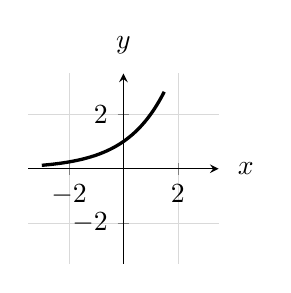
\begin{tikzpicture}
\begin{axis}[
    width=4cm, height=4cm,
    axis lines=middle,
    xmin=-3, xmax=3,
    ymin=-3, ymax=3,
    xtick={-2, 2}, ytick={-2, 2},
    grid=both,
    grid style={line width=.1pt, draw=gray!30},
    enlargelimits={abs=0.5},
    xlabel={$x$}, ylabel={$y$},
    every axis x label/.style={at={(ticklabel* cs:1.05)}, anchor=west},
    every axis y label/.style={at={(ticklabel* cs:1.05)}, anchor=south},
]
\addplot[domain=-3:1.5, samples=50, line width=1.2pt] {2^x};
\end{axis}
\end{tikzpicture}
\quad
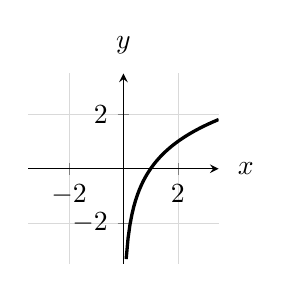
\begin{tikzpicture}
\begin{axis}[
    width=4cm, height=4cm,
    axis lines=middle,
    xmin=-3, xmax=3,
    ymin=-3, ymax=3,
    xtick={-2, 2}, ytick={-2, 2},
    grid=both,
    grid style={line width=.1pt, draw=gray!30},
    enlargelimits={abs=0.5},
    xlabel={$x$}, ylabel={$y$},
    every axis x label/.style={at={(ticklabel* cs:1.05)}, anchor=west},
    every axis y label/.style={at={(ticklabel* cs:1.05)}, anchor=south},
]
\addplot[domain=0.1:3.5, samples=50, line width=1.2pt] {ln(x)/ln(2)};
\end{axis}
\end{tikzpicture}
\quad
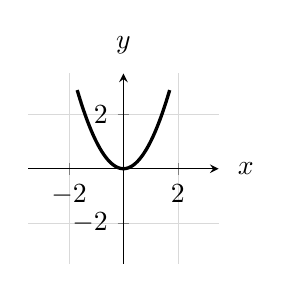
\begin{tikzpicture}
\begin{axis}[
    width=4cm, height=4cm,
    axis lines=middle,
    xmin=-3, xmax=3,
    ymin=-3, ymax=3,
    xtick={-2, 2}, ytick={-2, 2},
    grid=both,
    grid style={line width=.1pt, draw=gray!30},
    enlargelimits={abs=0.5},
    xlabel={$x$}, ylabel={$y$},
    every axis x label/.style={at={(ticklabel* cs:1.05)}, anchor=west},
    every axis y label/.style={at={(ticklabel* cs:1.05)}, anchor=south},
]
\addplot[domain=-1.7:1.7, samples=50, line width=1.2pt] {x^2};
\end{axis}
\end{tikzpicture}
\end{center}

\textbf{A.} Which two graphs represent the inverse of each other? Explain.

\textbf{B. Look for Relationships} What is the relationship between the domain and the range of the two inverse relations? \textbf{MP.7}
\end{model-discuss}

\begin{example}{1}
\textbf{Identify Key Features of Logarithmic Functions}

Graph $g(x) = \log_2 x$. What are the domain, range, $x$-intercept, and asymptote? What is the end behavior of the graph?

Logarithmic functions are inverse of exponential functions. Create tables of values for $f(x) = 2^x$ and $g(x) = \log_2 x$.

\begin{center}
\begin{tabular}{|c|c|c|c|c|c|}
\hline
$f(x)$ & $-2$ & $-1$ & $0$ & $1$ & $2$ \\
\hline
$y$ & $\frac{1}{4}$ & $\frac{1}{2}$ & $1$ & $2$ & $4$ \\
\hline
\end{tabular}
\quad
\begin{tabular}{|c|c|c|c|c|c|}
\hline
$g(x)$ & $\frac{1}{4}$ & $\frac{1}{2}$ & $1$ & $2$ & $4$ \\
\hline
$y$ & $-2$ & $-1$ & $0$ & $1$ & $2$ \\
\hline
\end{tabular}
\end{center}

\begin{concept-box}
\textbf{LOOK FOR RELATIONSHIPS}
For each key feature of the logarithmic function, state the corresponding key feature of the exponential function. \textbf{MP.7}
\end{concept-box}

Graph the functions and note the key features of $g(x)$.

\begin{center}
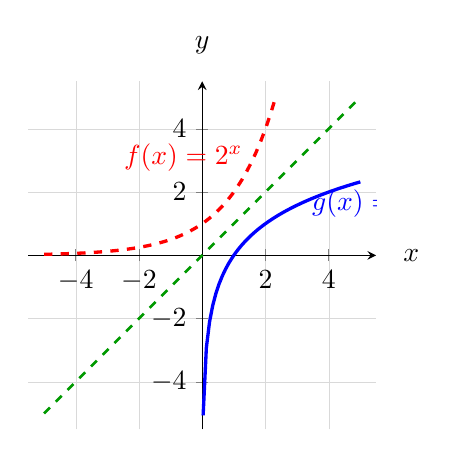
\begin{tikzpicture}
\begin{axis}[
    width=6cm, height=6cm,
    axis lines=middle,
    xmin=-5, xmax=5,
    ymin=-5, ymax=5,
    xtick={-4, -2, 2, 4}, ytick={-4, -2, 2, 4},
    grid=both,
    grid style={line width=.1pt, draw=gray!30},
    enlargelimits={abs=0.5},
    xlabel={$x$}, ylabel={$y$},
    every axis x label/.style={at={(ticklabel* cs:1.05)}, anchor=west},
    every axis y label/.style={at={(ticklabel* cs:1.05)}, anchor=south},
]
\addplot[domain=-5:5, samples=20, dashed, green!60!black, line width=1pt] {x};
\addplot[domain=-5:2.3, samples=50, dashed, red, line width=1.2pt] {2^x} node[pos=0.8, left] {$f(x) = 2^x$};
\addplot[domain=0.03:5, samples=50, blue, line width=1.2pt] {ln(x)/ln(2)} node[pos=0.8, right] {$g(x) = \log_2 x$};
\end{axis}
\end{tikzpicture}
\end{center}

\begin{itemize}
    \item domain: $\{x \mid x > 0\}$
    \item range: all real numbers
    \item $x$-intercept: $1$
    \item asymptote: $y$-axis
    \item end behavior: As $x \to 0, y \to -\infty$. As $x \to \infty, y \to \infty$.
\end{itemize}

Callouts:
\begin{itemize}
    \item The functions $f$ and $g$ are inverse functions. The graphs are reflections of each other across the line $y = x$.
    \item Notice the ordered pairs reinforce that the functions are inverses.
    \item The logarithmic function accepts only positive input values.
    \item The graph of the logarithmic function approaches $x = 0$ but does not touch it.
\end{itemize}
\end{example}

\begin{tryit}{1}
Graph each function and identify the domain and range. List any intercepts or asymptotes. Describe the end behavior.

a. $y = \ln x$ \qquad b. $y = \log_{\frac{1}{2}} x$
\end{tryit}

\begin{example}{2}
\textbf{Graph Transformations of Logarithmic Functions}

Graph the function $g(x) = \log_2(x + 3)$. How do the asymptote and $x$-intercept of the given function compare to those of the parent function $f(x) = \log_2 x$?

$f(x) = \log_2 x$

$g(x) = \log_2(x + 3) = f(x - (-3))$

Since $g(x) = f(x + 3)$, then $g$ is the logarithmic function translated $3$ units to the left. 

The vertical asymptote and the $x$-intercept each shift $3$ units to the left.

\begin{center}
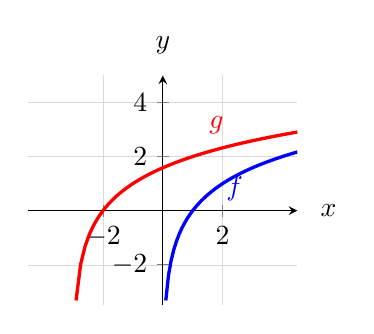
\begin{tikzpicture}
\begin{axis}[
    width=5cm, height=4.5cm,
    axis lines=middle,
    xmin=-4, xmax=4,
    ymin=-3, ymax=4.5,
    xtick={-2, 2}, ytick={-2, 2, 4},
    grid=both,
    grid style={line width=.1pt, draw=gray!30},
    enlargelimits={abs=0.5},
    xlabel={$x$}, ylabel={$y$},
    every axis x label/.style={at={(ticklabel* cs:1.05)}, anchor=west},
    every axis y label/.style={at={(ticklabel* cs:1.05)}, anchor=south},
]
\addplot[domain=0.1:4.5, samples=50, blue, line width=1.2pt] {ln(x)/ln(2)} node[pos=0.6, right] {$f$};
\addplot[domain=-2.9:4.5, samples=50, red, line width=1.2pt] {ln(x+3)/ln(2)} node[pos=0.8, above left] {$g$};
\end{axis}
\end{tikzpicture}
\end{center}

\begin{concept-box}
\textbf{REASON}
Consider the transformation of a parent function translated by $(h, k)$ so that $g(x) = f(x + h) + k$. With exponential functions, the value of $k$ dictates the shift of the horizontal asymptote. With logarithmic functions, the value of $h$ determines the shift of the asymptote.
\end{concept-box}
\end{example}

\begin{tryit}{2}
Describe how each graph compares to the graph of $f(x) = \ln x$.

a. $g(x) = \ln x + 4$ \qquad b. $h(x) = 5 \ln x$
\end{tryit}

\begin{example}{3}
\textbf{Inverses of Exponential and Logarithmic Functions}

What is the equation of the inverse of the functions?

\textbf{A. $f(x) = 10^{x+1}$}
\begin{align*}
y &= 10^{x+1} \\
x &= 10^{y+1} \quad \text{(Rewrite the function as $y=$, interchange $x$ and $y$, and solve for $y$.)} \\
y + 1 &= \log x \\
y &= \log x - 1
\end{align*}
The equation of the inverse of $f(x) = 10^{x+1}$ is $f^{-1}(x) = \log x - 1$.

Verify by function composition.
\begin{align*}
f(f^{-1}(x)) &= 10^{(\log x - 1) + 1} & f^{-1}(f(x)) &= \log 10^{x+1} - 1 \\
&= 10^{\log x} & &= x + 1 - 1 \\
&= x & &= x
\end{align*}

\begin{center}
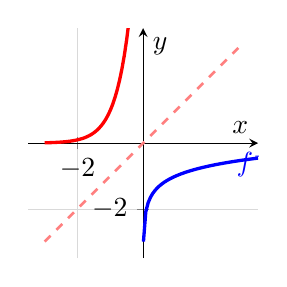
\begin{tikzpicture}
\begin{axis}[
    width=4.5cm, height=4.5cm,
    axis lines=middle,
    xmin=-3, xmax=3,
    ymin=-3, ymax=3,
    xtick={-2}, ytick={-2},
    grid=both,
    grid style={line width=.1pt, draw=gray!30},
    enlargelimits={abs=0.5},
    xlabel={$x$}, ylabel={$y$},
]
\addplot[domain=-3:3, samples=20, dashed, red!50!white, line width=1pt] {x};
\addplot[domain=-3:0.5, samples=50, red, line width=1.2pt] {10^(x+1)} node[pos=0.8, left] {$f$};
\addplot[domain=0.01:3.5, samples=50, blue, line width=1.2pt] {log10(x)-1} node[pos=0.8, right] {$f^{-1}$};
\end{axis}
\end{tikzpicture}
\end{center}

\begin{concept-box}
\textbf{CONCEPTUAL UNDERSTANDING} \\
\textbf{LOOK FOR RELATIONSHIPS} \\
$f(x)$ is a translation of the parent function $y = 10^x$ one unit left. $f^{-1}(x)$ is a translation of the parent function $y = \log x$ one unit down. Graphical translations of a function and its inverse are directly related. Explain.
\end{concept-box}

\textbf{B. $g(x) = \log_7(x + 5)$}
\begin{align*}
y &= \log_7(x + 5) \quad \text{(Rewrite as $y=$.)} \\
x &= \log_7(y + 5) \\
y + 5 &= 7^x \\
y &= 7^x - 5
\end{align*}
The equation of the inverse of $g(x) = \log_7(x + 5)$ is $g^{-1}(x) = 7^x - 5$.

Verify by function composition.
\begin{align*}
g(g^{-1}(x)) &= \log_7(7^x - 5 + 5) & g^{-1}(g(x)) &= 7^{\log_7(x + 5)} - 5 \\
&= \log_7 7^x & &= x + 5 - 5 \\
&= x & &= x
\end{align*}

\begin{center}
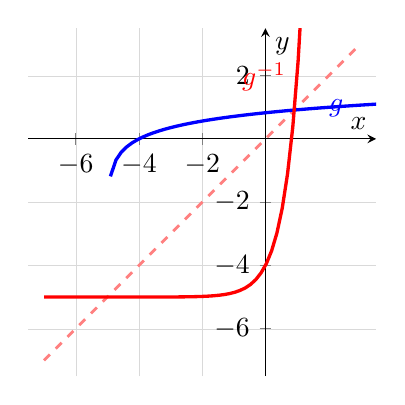
\begin{tikzpicture}
\begin{axis}[
    width=6cm, height=6cm,
    axis lines=middle,
    xmin=-7, xmax=3,
    ymin=-7, ymax=3,
    xtick={-6, -4, -2}, ytick={-6, -4, -2, 2},
    grid=both,
    grid style={line width=.1pt, draw=gray!30},
    enlargelimits={abs=0.5},
    xlabel={$x$}, ylabel={$y$},
]
\addplot[domain=-7:3, samples=20, dashed, red!50!white, line width=1pt] {x};
\addplot[domain=-4.9:3.5, samples=50, blue, line width=1.2pt] {ln(x+5)/ln(7)} node[pos=0.8, right] {$g$};
\addplot[domain=-7:1.2, samples=50, red, line width=1.2pt] {7^x - 5} node[pos=0.8, left] {$g^{-1}$};
\end{axis}
\end{tikzpicture}
\end{center}
\end{example}

\begin{tryit}{3}
Find the inverse of each function. Then verify they are inverses by composition.

a. $f(x) = 3^{x+2}$ \qquad b. $g(x) = \log_7 x - 2$
\end{tryit}

\begin{example}{4}
\textbf{Use a Logarithmic Function as a Model}

A logarithmic function can approximate the altitude of a plane over time.

\placeholder{photo}{Airplane taking off with callouts: $A = 9,200 \ln t + 10,000$. $t$ is time in minutes after take off. $A$ is altitude in feet.}

\textbf{A. What is the altitude of the plane 10 minutes after takeoff?}

Substitute 10 for $t$ in the equation of the function.
\begin{align*}
A &= 9,200 \ln 10 + 10,000 \\
&\approx 9,200(2.303) + 10,000 \\
&\approx 21,188 + 10,000 \\
&\approx 31,188
\end{align*}
After 10 minutes, the plane's altitude is about 31,188 feet.

\textbf{B. How long after takeoff will the plane reach an altitude of 35,000 feet?}

Rearrange the equation to isolate the variable $t$.
\begin{align*}
A &= 9,200 \ln t + 10,000 \\
A - 10,000 &= 9,200 \ln t \\
\frac{A - 10,000}{9,200} &= \ln t \\
t &= e^{\left(\frac{A - 10,000}{9,200}\right)}
\end{align*}

In the rearranged equation, time is a function of altitude, so use substitution to find time.
\begin{align*}
t &= e^{\left(\frac{35,000 - 10,000}{9,200}\right)} \\
&\approx 15.14
\end{align*}
The plane will reach an altitude of 35,000 feet after about 15.14 minutes.

\textbf{C. Evaluate the model against the altitude of the plane.}

On the domain interval $(0, 0.337)$ the logarithmic function is negative. The altitude of the plane is not correct during this interval. Also, the plane starts at the origin, which is on the asymptote of the model.

\begin{concept-box}
\textbf{STUDY TIP}
The original equation is a logarithmic function, while the rearranged equation is an exponential function. The exponential function is the inverse of the logarithmic function.
\end{concept-box}
\end{example}

\begin{tryit}{4}
Commercial airplanes usually fly no higher than 38,000 ft. How long will it take the plane to reach this altitude? How does a maximum cruising height compare with the model?
\end{tryit}

\begin{concept-summary}
\textbf{Logarithmic Functions}

\begin{tabular}{p{3cm} p{4cm} p{4cm}}
\toprule
\textbf{GRAPH} & 
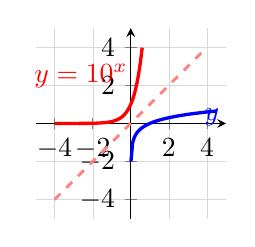
\begin{tikzpicture}[baseline=(current bounding box.center)]
\begin{axis}[
    width=4cm, height=4cm,
    axis lines=middle,
    xmin=-4.5, xmax=4.5,
    ymin=-4.5, ymax=4.5,
    xtick={-4, -2, 2, 4}, ytick={-4, -2, 2, 4},
    grid=both,
    grid style={line width=.1pt, draw=gray!30},
    enlargelimits={abs=0.5},
]
\addplot[domain=-4:4, samples=20, dashed, red!50!white, line width=1pt] {x};
\addplot[domain=-4:0.6, samples=50, red, line width=1.2pt] {10^x} node[pos=0.8, left] {$y = 10^x$};
\addplot[domain=0.01:4.5, samples=50, blue, line width=1.2pt] {log10(x)} node[pos=0.8, right] {$y = \log x$};
\end{axis}
\end{tikzpicture}
&
The functions are inverses so their graphs are reflections of each other across the line with equation $y = x$. \\
\midrule
\textbf{EQUATIONS} & $y = \log x$ & $y = 10^x$ \\
\midrule
\textbf{KEY FEATURES} & 
Domain: $\{x \mid x > 0\}$ \par Range: all real numbers \par $x$-intercept: $1$ \par Asymptote: $y$-axis & 
Domain: \textit{all real numbers} \par Range: $\{y \mid y > 0\}$ \par $y$-intercept: $1$ \par Asymptote: $x$-axis \\
\midrule
\textbf{END BEHAVIOR} & 
As $x \to 0, y \to -\infty$ \par As $x \to \infty, y \to \infty$ &
As $x \to -\infty, y \to 0$ \par As $x \to \infty, y \to \infty$ \\
\bottomrule
\end{tabular}
\end{concept-summary}

\vspace{1em}
\textbf{Do You UNDERSTAND?}

\begin{practice}{1}{}
\textbf{ESSENTIAL QUESTION} How is the relationship between logarithmic and exponential functions revealed in the key features of their graphs?
\answer{}
\end{practice}

\begin{practice}{2}{}
\textbf{Error Analysis} Raynard claims the domain of the function $y = \log_3 x$ is all real numbers. Explain the error Raynard made.
\answer{}
\end{practice}

\begin{practice}{3}{}
\textbf{Communicate Precisely} How are the graphs of $f(x) = \log_5 x$ and $g(x) = -\log_5 x$ related?
\answer{}
\end{practice}

\begin{practice}{4}{}
\textbf{Use Structure} Explain the necessary steps to find the inverse of $h(x) = \log_6(x + 4)$.
\answer{}
\end{practice}

\vspace{1em}
\textbf{Do You KNOW HOW?}

\begin{practice}{5}{}
Graph the function $y = \log_4 x$ and identify the domain and range. List any intercepts or asymptotes. Describe the end behavior.
\answer{}
\end{practice}

\begin{practice}{6}{}
Write the equation for the function $g(x)$, which can be described as a vertical shift $1\frac{1}{2}$ units up from the function $f(x) = \ln x - 1$.
\answer{}
\end{practice}

\begin{practice}{7}{}
The function $y = 5 \ln(x + 1)$ gives $y$, the number of downloads, in hundreds, $x$ minutes after the release of a song. Find the equation of the inverse and interpret its meaning.

\placeholder{diagram}{Downloading progress bar labeled 'Downloading...' with 'y downloads' and 'x minutes'.}
\answer{}
\end{practice}

\begin{practice}{8}{}
Sketch the functions represented by the tables. Identify which graph is the logarithmic function. Are the two functions inverses?

\textbf{a.}
\begin{tabular}{|c|c|c|c|c|c|}
\hline
$x$ & $10^{-10}$ & $0.01$ & $1$ & $2$ & $10$ \\
\hline
$g(x)$ & $-8$ & $0$ & $2$ & $2.301$ & $3$ \\
\hline
\end{tabular}

\textbf{b.}
\begin{tabular}{|c|c|c|c|c|c|c|}
\hline
$x$ & $-1$ & $0$ & $1$ & $2$ & $3$ & $4$ \\
\hline
$h(x)$ & $0.001$ & $0.01$ & $0.1$ & $1$ & $10$ & $100$ \\
\hline
\end{tabular}
\answer{}
\end{practice}

\vspace{2em}
\textbf{PRACTICE \& PROBLEM SOLVING}

\textbf{UNDERSTAND}

\begin{practice}{9}{}
\textbf{Look for Relationships} Are the logarithmic and exponential functions shown inverses of each other? Explain.

\begin{center}
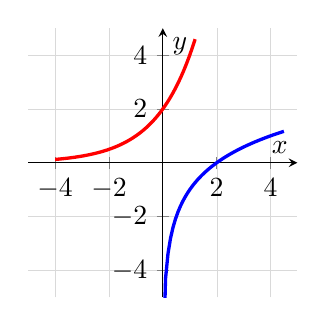
\begin{tikzpicture}
\begin{axis}[
    width=5cm, height=5cm,
    axis lines=middle,
    xmin=-4.5, xmax=4.5,
    ymin=-4.5, ymax=4.5,
    xtick={-4, -2, 2, 4}, ytick={-4, -2, 2, 4},
    grid=both,
    grid style={line width=.1pt, draw=gray!30},
    enlargelimits={abs=0.5},
    xlabel={$x$}, ylabel={$y$},
]
\addplot[domain=-4:1.2, samples=50, red, line width=1.2pt] {2^(x+1)};
\addplot[domain=0.01:4.5, samples=50, blue, line width=1.2pt] {ln(x)/ln(2) - 1};
\end{axis}
\end{tikzpicture}
\end{center}
\answer{}
\end{practice}

\begin{practice}{10}{}
\textbf{Communicate Precisely} How is the graph of the logarithmic function $g(x) = \log_2(x-7)$ related to the graph of the function $f(x) = \log_2 x$? Explain your reasoning.
\answer{}
\end{practice}

\begin{practice}{11}{}
\textbf{Error Analysis} Describe and correct the error a student made in finding the inverse of the exponential function $f(x) = 5^{x-6} + 2$.

\begin{center}
\begin{tabular}{ll}
$y = 5^{x-6} + 2$ & Write in $y = f(x)$ form. \\
$x = 5^{y-6} + 2$ & Interchange $x$ and $y$. \\
$x - 2 = 5^{y-6}$ & Subtract $2$ from each side. \\
$y - 6 = \log_5 x - 2$ & Rewrite in logarithmic form. \\
$y = \log_5 x - 2 + 6$ & Add $6$ to each side. \\
$y = \log_5 x + 4$ & Simplify. \\
$f'(x) = \log_5 x + 4$ & \placeholder{diagram}{Red X marking the work as incorrect.}
\end{tabular}
\end{center}
\answer{}
\end{practice}

\begin{practice}{12}{}
\textbf{Make Sense and Persevere} The number of members $m$ who joined a new workout center $w$ weeks after opening is modeled by the equation $m = 1.6^{w+2}$, where $0 \leq w \leq 10$. Find the inverse of the function and explain what the inverse tells you.
\answer{}
\end{practice}

\begin{practice}{13}{}
\textbf{Use Structure} The graph shows a transformation of the parent graph $f(x) = \log_3 x$. Write an equation for the graph.

\begin{center}
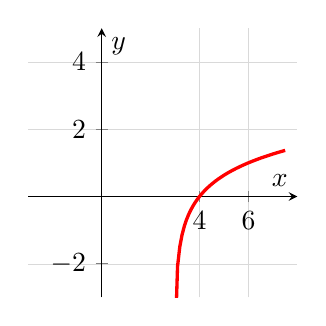
\begin{tikzpicture}
\begin{axis}[
    width=5cm, height=5cm,
    axis lines=middle,
    xmin=-2.5, xmax=7.5,
    ymin=-2.5, ymax=4.5,
    xtick={4, 6}, ytick={-2, 2, 4},
    grid=both,
    grid style={line width=.1pt, draw=gray!30},
    enlargelimits={abs=0.5},
    xlabel={$x$}, ylabel={$y$},
]
\addplot[domain=3.01:7.5, samples=50, red, line width=1.2pt] {ln(x-3)/ln(3)};
\end{axis}
\end{tikzpicture}
\end{center}
\answer{}
\end{practice}

\vspace{1em}
\textbf{PRACTICE}

Graph each function and identify the domain and range. List any intercepts or asymptotes. Describe the end behavior. \textbf{SEE EXAMPLE 1}

\begin{practice}{14}{}
$y = \log_5 x$
\answer{}
\end{practice}

\begin{practice}{15}{}
$y = \log_8 x$
\answer{}
\end{practice}

\begin{practice}{16}{}
$y = \log_{\frac{3}{10}} x$
\answer{}
\end{practice}

\begin{practice}{17}{}
$y = \log_{0.1} x$
\answer{}
\end{practice}

Describe the graph in terms of transformations of the parent function $f(x) = \log_6 x$. Compare the asymptote and $x$-intercept of the given function to the parent function. \textbf{SEE EXAMPLE 2}

\begin{practice}{18}{}
$g(x) = \frac{1}{2} \log_6 x$
\answer{}
\end{practice}

\begin{practice}{19}{}
$g(x) = \log_6 (-x)$
\answer{}
\end{practice}

\begin{practice}{20}{}
Describe how the graph of $g(x) = -\ln(x + 0.5)$ is related to the graph of $f(x) = \ln x$. \textbf{SEE EXAMPLE 2}
\answer{}
\end{practice}

Find the equation of the inverse of each function. \textbf{SEE EXAMPLE 3}

\begin{practice}{21}{}
$f(x) = 5^{x-3}$
\answer{}
\end{practice}

\begin{practice}{22}{}
$f(x) = \left(\frac{1}{2}\right)^{x-1}$
\answer{}
\end{practice}

\begin{practice}{23}{}
$f(x) = 6^{x+7}$
\answer{}
\end{practice}

\begin{practice}{24}{}
$f(x) = \log_2 (8x)$
\answer{}
\end{practice}

\begin{practice}{25}{}
$f(x) = \ln (x + 3) - 1$
\answer{}
\end{practice}

\begin{practice}{26}{}
$f(x) = 4 \log_2 (x - 3) + 2$
\answer{}
\end{practice}

\begin{practice}{27}{}
The altitude $y$, in feet, of a plane $t$ minutes after takeoff is approximated by the function $y = 5,000 \ln(.05t) + 8,000$. Solve for $t$ in terms of $y$. What is a situation in which it would be easier to use your new equation rather than the original? \textbf{SEE EXAMPLE 4}
\answer{}
\end{practice}

\begin{practice}{28}{}
A company uses this function to relate sales revenue, $R$, and advertising costs, $a$. What is the equation of the inverse of the equation? Which equation would be easier to use to find a value of $a$ for a particular value of $R$? \textbf{SEE EXAMPLE 4}

\placeholder{diagram}{Block diagram. Sales Revenue, R pointing via an arrow with a \$ symbol, and Advertising Costs, a pointing via an arrow with 'ADS'. Function reads $R = 12 \log(a + 1) + 25$.}
\answer{}
\end{practice}

\vspace{1em}
\textbf{APPLY}

\begin{practice}{29}{}
\textbf{Model with Mathematics} The equation $r = 90 - 25 \log(t + 1)$ is to model a student's retention $r$ after taking a physics course where $r$ represents a student's test score (as a percent), and $t$ represents the number of months since taking the course.

\textbf{a.} Make a table of values for ordered pairs that represent $r = 90 - 25 \log(t + 1)$, rounding to the nearest tenth. Then sketch the graph of the function on a coordinate plane through those ordered pairs. (You may use a graphing calculator to check.)

\textbf{b.} Find the equation of the inverse. Interpret the meaning of this function.
\answer{}
\end{practice}

\begin{practice}{30}{}
\textbf{Higher Order Thinking} As shown by the diagram, an earthquake occurs below Earth's surface at point $F$ (the focus). Point $E$, on the surface above the focus, is called the \textit{epicenter}. A seismograph station at point $S$ records the waves of energy generated by the earthquake. The surface wave magnitude $M$ of the earthquake is given by this formula:
$$M = \log\left(\frac{A}{T}\right) + 1.66(\log D) + 3.3$$
In the formula, $A$ is the amplitude of the ground motion in micrometers, $T$ is the period in seconds, and $D$ is the measure of $\angle ES$ in degrees.

\placeholder{diagram}{Cross section of the Earth. Epicenter $E$ is on the surface. Focus $F$ is directly below $E$. Seismograph Station $S$ is on the surface at some distance from $E$.}

\textbf{a.} Find surface wave magnitude of an earthquake with $A = 700$ micrometers, $T = 2$ and $D = 100^\circ$.

\textbf{b.} In the formula, $20^\circ < D \leq 160^\circ$. By how much can the size of arc $ES$ affect the surface wave magnitude? Explain.
\answer{}
\end{practice}

\vspace{1em}
\textbf{ASSESSMENT PRACTICE}

\begin{practice}{31}{}
The logarithmic function $g(x) = \ln x$ is transformed to $h(x) = \ln(x + 2) - 1$. Which of the following are true? Select all that apply.
\begin{itemize}
    \item[$\square$] $g(x)$ is translated $2$ units upward.
    \item[$\square$] $g(x)$ is translated $2$ units to the right.
    \item[$\square$] $g(x)$ is translated $2$ units to the left.
    \item[$\square$] $g(x)$ is translated $1$ unit downward.
    \item[$\square$] $g(x)$ is translated $1$ unit to the left.
    \item[$\square$] The vertical asymptote shifts $2$ units to the left.
    \item[$\square$] The vertical asymptote shifts $2$ units to the right.
\end{itemize}
\answer{}
\end{practice}

\begin{practice}{32}{}
\textbf{SAT/ACT} The graph shows the exponential function $f(x) = 5^{x+1}$. Which of the following functions represents its inverse, $f^{-1}(x)$?

\begin{center}
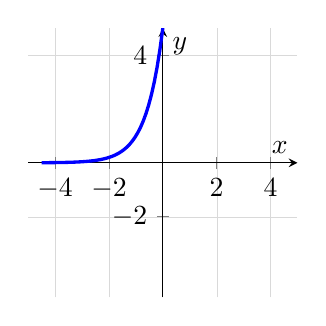
\begin{tikzpicture}
\begin{axis}[
    width=5cm, height=5cm,
    axis lines=middle,
    xmin=-4.5, xmax=4.5,
    ymin=-4.5, ymax=4.5,
    xtick={-4, -2, 2, 4}, ytick={-2, 4},
    grid=both,
    grid style={line width=.1pt, draw=gray!30},
    enlargelimits={abs=0.5},
    xlabel={$x$}, ylabel={$y$},
]
\addplot[domain=-4.5:0.5, samples=50, blue, line width=1.2pt] {5^(x+1)};
\end{axis}
\end{tikzpicture}
\end{center}

\begin{tabular}{ll}
\textcircled{A} $f^{-1}(x) = 1 + \log_5 x$ & \textcircled{B} $f^{-1}(x) = \log_5 x - 1$ \\
\textcircled{C} $f^{-1}(x) = \log_5 (x - 1)$ & \textcircled{D} $f^{-1}(x) = \log_5 (x + 1)$
\end{tabular}
\answer{}
\end{practice}

\begin{practice}{33}{}
\textbf{Performance Task} The logarithmic function $M(d) = 5 \log d + 2$ is used to find the limiting magnitude of a telescope, where $d$ represents the diameter of the lens of the telescope (mm) that is being used for the observation.

\textbf{Part A} Find the limiting magnitude of a telescope having a lens diameter of $40$ mm.

\textbf{Part B} Find the equation of the inverse of this function.

\textbf{Part C} Interpret why astronomers may wish to use the inverse of this function. Justify your reasoning.

\textbf{Part D} Using the inverse function, find the diameter of the lens that has a limiting magnitude of $13.5$. Check your answer with the table function of your graphing calculator.
\answer{}
\end{practice}

\end{document}